\section{CHAPTER 10: ETP\cite{etp}}
\begin{figure}[h!]
    \centering
    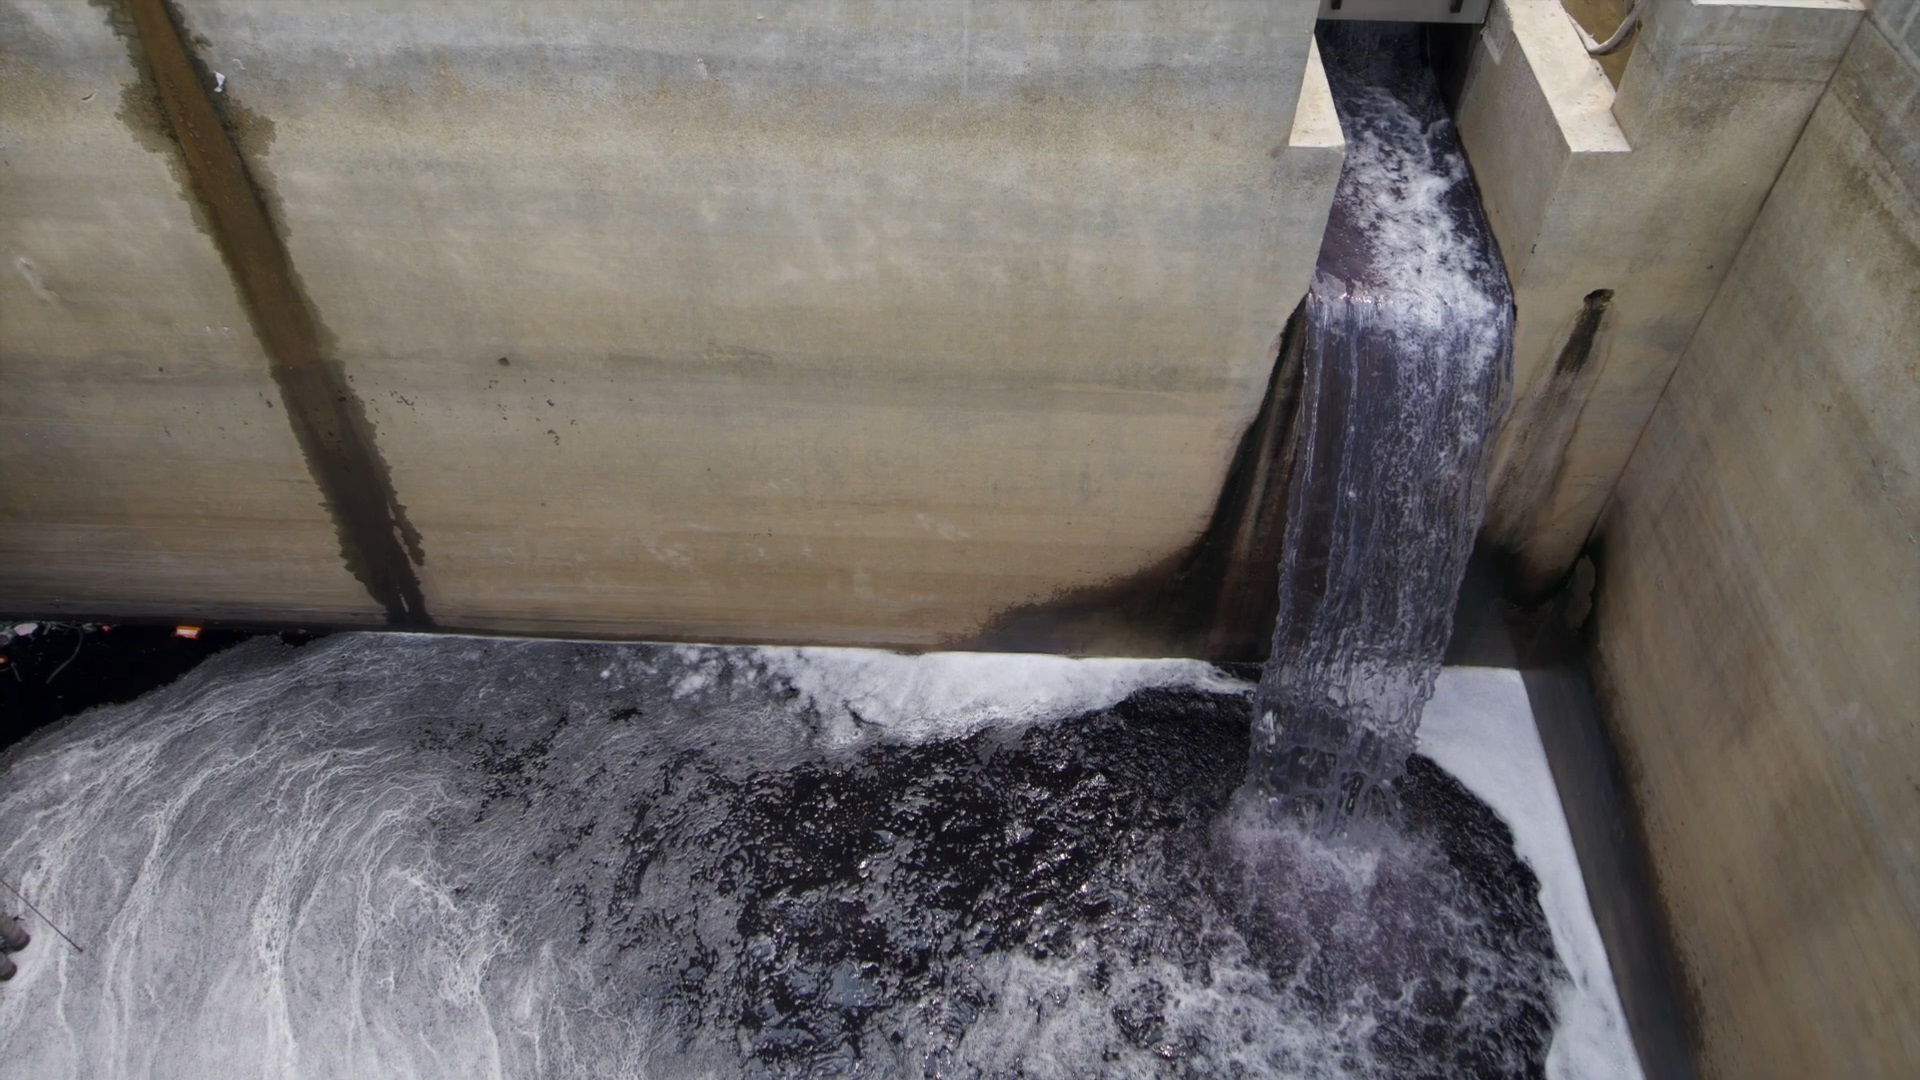
\includegraphics[width=1\linewidth]{figs/etp.jpg}
    \caption{ETP (Top) at the Industrial Tour}
    \label{fig:etp}
\end{figure}

\begin{figure}[h!]
    \centering
    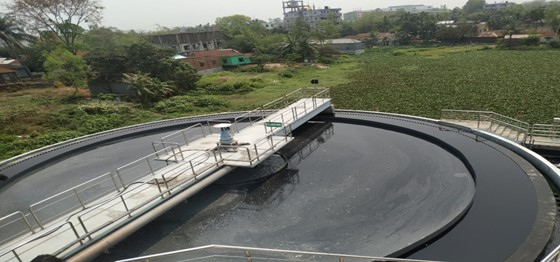
\includegraphics[width=1\linewidth]{figs/etp2.jpg}
    \caption{ETP (Bottom) at the Industrial Tour}
    \label{fig:etp2}
\end{figure}

Effluent treatment plant, also known as ETP is a waste water treatment process (WWTP) that is used to treat waste water. It is mostly used in industries like pharmaceuticals, textiles, and chemicals where extreme water contamination is a possibility. Figure \ref{fig:etp} and \ref{fig:etp2} are from textile industry.

Effluent Treatment Plant plays a significant role in the treatment of industrial waste water as well as domestic sewage. Organic matter, inorganic matter, heavy metals, oil \& grease, suspended particles, and other contaminants are treated in the wastewater treatment process of an ETP plant. 

The treatment includes the removal of suspended particles, dissolved organic matters and handling of sludge for disposal.

The process may be a chemical one, biological one or a combination of biological and chemical one. Figure \ref{fig:etp} and \ref{fig:etp2} are both of biological type.

Equalisation: The equalization tank's purpose is to balance the raw effluent from various processing units. The wastewater is collected in an existing mixed effluent tank and pumped to an existing aeration tank, which also functions as an equalisation tank. The floating aerator is used to homogenise the effluent before it is pumped to the neutralization tank for treatment.
pH control: The pH value of effluent should be between 5.5 and 9.0, according to the Bureau of Indian Standards (BIS). pH neutralization is used to modify the pH of waste water.
For waste that is acidic (low pH): Bases are used to modify the pH of a solution.
In the case of alkali waste (high pH): Acids are used to modify the pH of a solution.
Coagulation: Coagulation is a technique that involves adding liquid aluminium sulphate to untreated water. This causes tiny dirt particles to stick together after mixing. This collection of particles combines to generate larger, heavier particles that are easily removed through settling and filtration.
Sedimentation: Water travels slowly in this process, causing the heavy particles to settle to the bottom. Sludge is the term for the particles that gather at the bottom of a container.

Filtration: Filtration is the process of passing water through a filter that removes particulates. The filters are made out of sand and gravel layers. Backwashing is required to clean these filters on a regular basis.
Disinfection: Before entering the distribution system, water is disinfected. Chlorine is used to disinfect and decontaminate water.

Sludge Drying: Sedimentation collects and settles down solids, which are then transported to drying beds. When the sludge thickness reaches around 300 mm, the sludge charging should be stopped, and the bed should be segregated to allow natural evaporation to dry it off. This takes approximately 10 days.

\begin{figure}[h!]
    \centering
    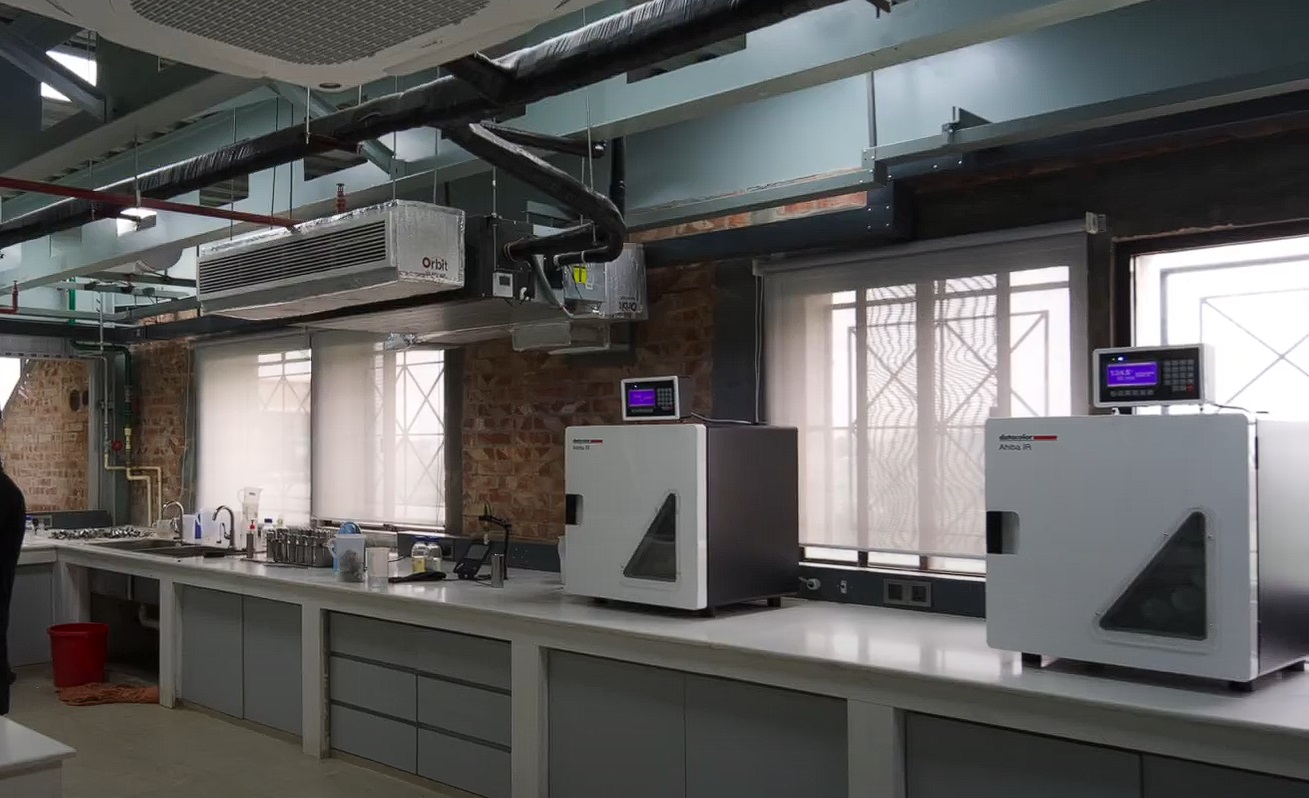
\includegraphics[width=0.8\linewidth]{figs/lab.jpg}
    \caption{LAB for measuring the condition of effluent water}
    \label{fig:LAB}
\end{figure}